\section{Results and Performance Analysis}

Operating across the hidden Neptune physics constraints, the accumulated testing phase results reveal the distinct operational trends afforded by the diverse ENA configuration modalities. Performance was quantified by averaging reliability thresholds across all 10 experimental runs.

\subsection{Online Testing Reliability \& Stability Gaps}
Across the four-world Testing sequence, varying success metrics illuminated explicit architectural gaps between the models. \textbf{ENA-03} achieved a marginally higher overarching Mean Reliability ($85.18\%$) compared to the pure Fuzzy-logic \textbf{ENA-01} ($84.91\%$) and Quadratic \textbf{ENA-02} baseline ($76.46\%$).

However, maximum absolute reliability does not translate to maximum \textit{adaptive stability}. To quantify shift-resilience, we calculated the ``Stability Gap"—defined as the mean score delta between the 20 episodes strictly preceding a gravitational shift and the 20 episodes immediately following it ($\Delta = \text{Score}_{pre} - \text{Score}_{post}$). An optimal transition gap approaches $0$, indicating the agent seamlessly retained baseline mastery without needing multi-episode transition recoveries.

Here, \textbf{ENA-01} out-scaled its counterparts. Operating purely on fuzzy mechanics, ENA-01 yielded a mathematical Stability Gap of only $-2.13$ ($\sigma = 4.66$). Because the second environment (Mars) physically allows higher survival intervals than Earth, negative values indicate expected score increases. ENA-01 transitioned smoothly with minimal variance. In contrast, ENA-03 demonstrated an inter-environment gap of $-20.89$ ($\sigma = 49.85$). This extremely high standard deviation on ENA-03 implies that aggressive quadratic trust-decay caused volatile behavior precisely during the transition boundary, whereas the fuzzy-logic configuration smoothed the evolutionary migration.

\begin{table}[htbp]
\caption{Testing Performance Across 10 Experiments (Without Significance Scaling)}
\begin{center}
\begin{tabular}{|c|c|c|c|c|}
\hline
\textbf{Configuration} & \textbf{Reliability} & \textbf{Rel. Std ($\sigma$)} & \textbf{Stability Gap} & \textbf{Gap Std ($\sigma$)} \\
\hline
ENA-01 & 84.91\% & 28.87\% & -2.13 & 4.66 \\
ENA-02 & 76.46\% & 21.14\% & -14.15 & 39.13 \\
ENA-03 & 85.18\% & 28.02\% & -20.89 & 49.85 \\
\hline
\end{tabular}
\label{tab:metrics}
\end{center}
\end{table}

\begin{figure}[htbp]
\centerline{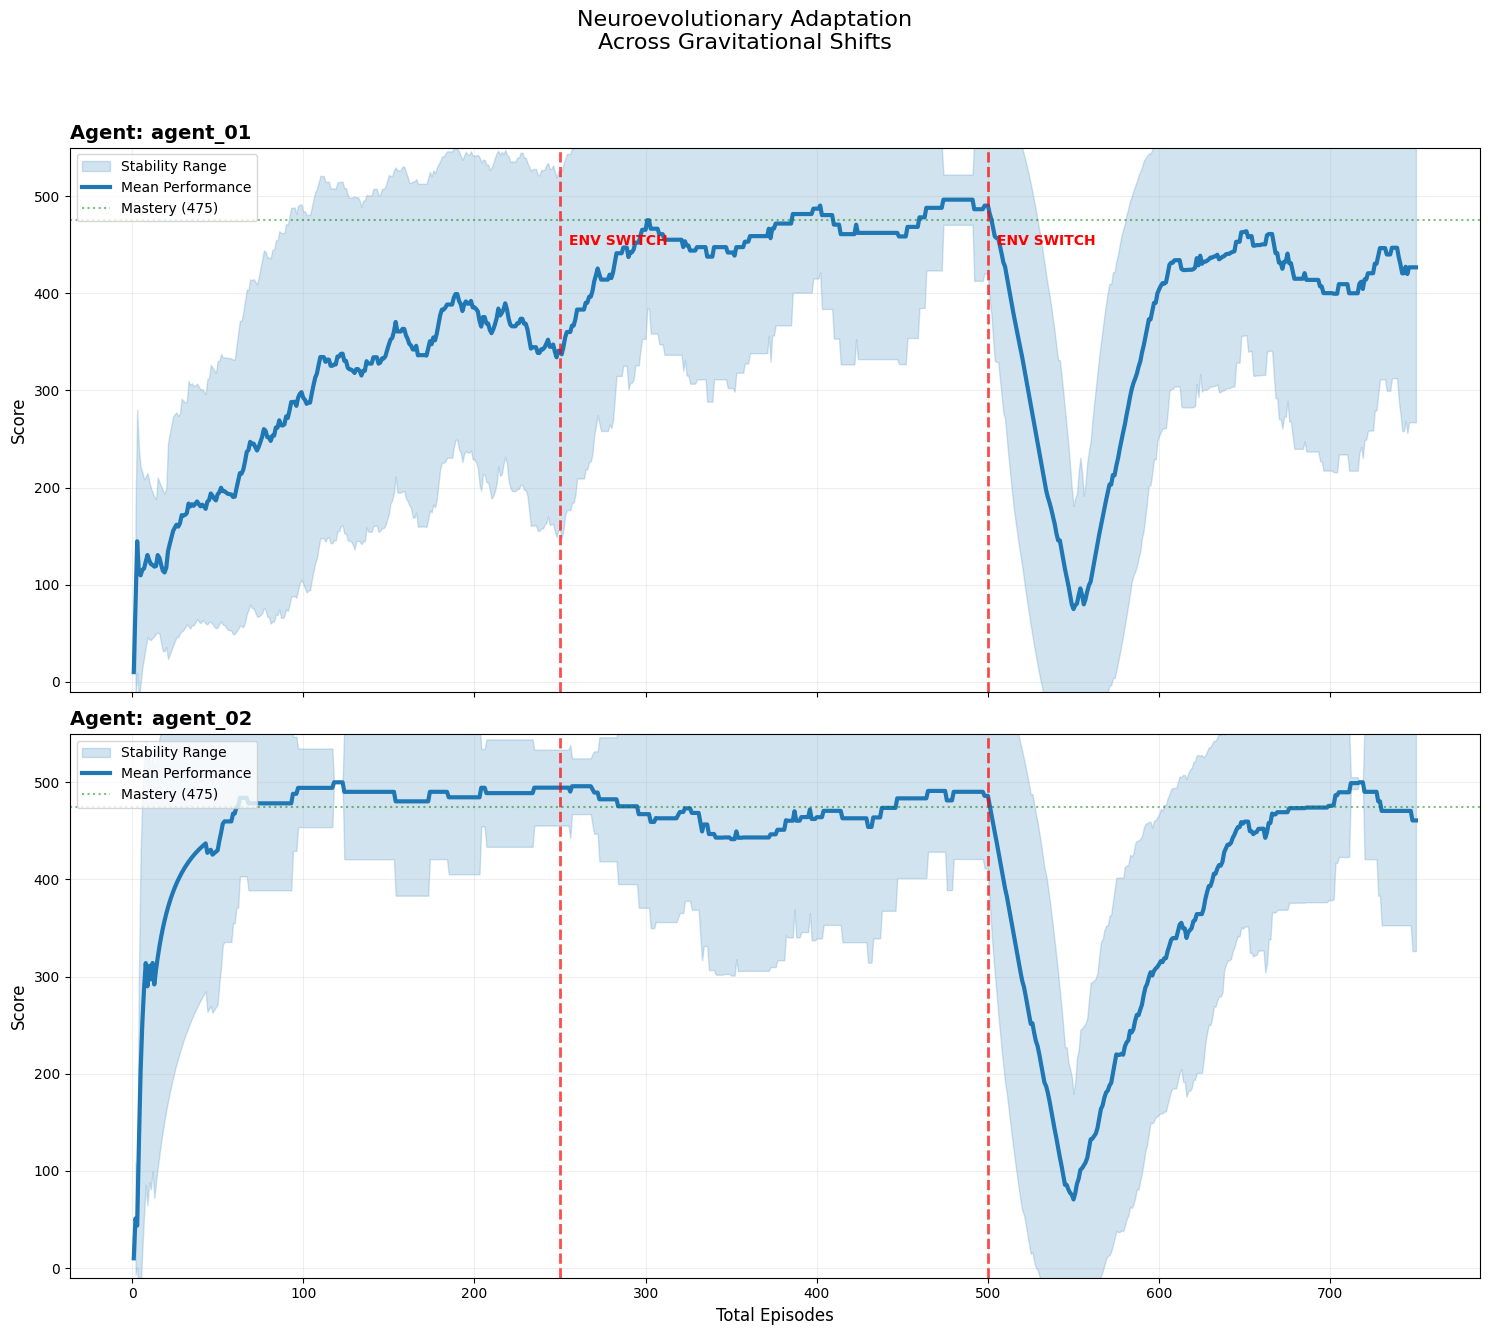
\includegraphics[width=\linewidth]{images/training_exp_01.png}}
\caption{Academic performance tracking the stability gap and deviation matrices over varying gravitational domain shifts (red markers).}
\label{fig:academic}
\end{figure}

\begin{figure}[htbp]
\centerline{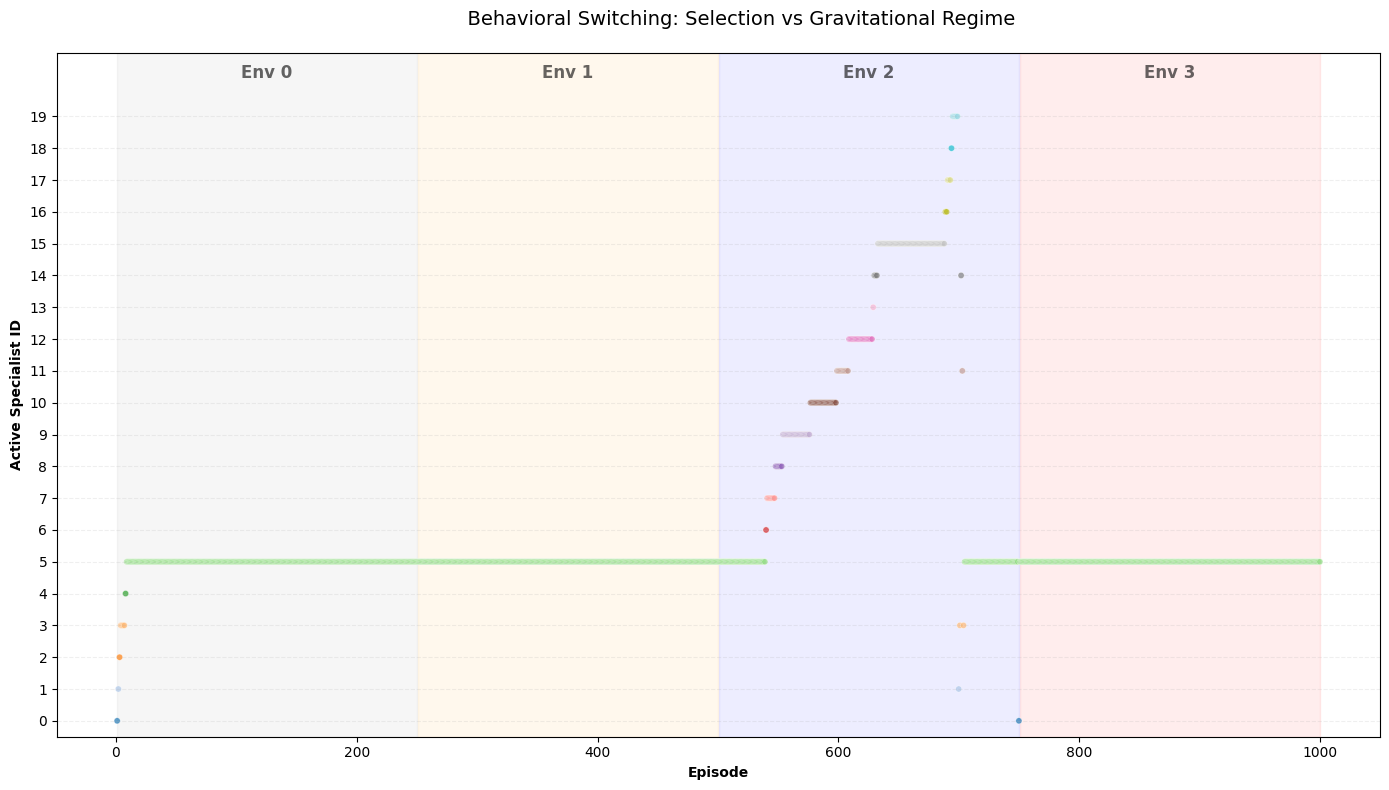
\includegraphics[width=\linewidth]{images/test_active_specialist_ena_01.png}}
\caption{Active Specialist behavioral switching matrix, directly plotting the specific Hall of Fame identity assumed sequence-to-sequence as the overarching gravitational parameters shift.}
\label{fig:specialist}
\end{figure}

\subsection{Initialization Variance and Evolutionary Constraints}
While ENA-01 demonstrated strong macroscopic testing generalizations, the 10 independent experiments strictly revealed profound macroscopic variance vulnerabilities. It is important to explicitly state that the vast standard deviations observed across merely 10 independent runs mathematically prohibit assigning strict statistical significance to the absolute superiority of ENA-01 over the baselines without future intensive t-test scaling; we analyze the outcomes here strictly as observed empirical trends.

Despite averaging an impressive $84.91\%$ reliability, ENA-01 reported an immense testing Standard Deviation ($\sigma = 28.87\%$). Analyzing individual experimental extrema revealed maximum testing mastery reaching a near-perfect $99.60\%$, abruptly contrasted by minimum catastrophic testing failures resolving at $0.80\%$ reliability.

This suggests that beneath constraints of a tiny localized computational window (population size $N=20$, absolute duration bound $250$ episodes), the Evolutionary Neuroplastic Agent remains highly reliant on the initial randomization matrices (often termed ``lucky" initializations). The $0.80\%$ test performance minimum highlights a potential mathematical vulnerability (pending future strict seed-control isolation studies): if initialized poorly, the limited ENA population narrowly overfits to its sequential training zones. Unable to properly illuminate the evolutionary space, the resultant Hall of Fame is physically unequipped to respond to hidden structural regimes like Neptune, resulting theoretically in localized test-time performance collapse.

\begin{figure}[htbp]
\centerline{
\includegraphics[width=\linewidth]{images/reliability_box.png}}
\caption{Box plot delineating the distribution spread of test-time Reliability across 10 randomized population initializations. The presence of single percentage extrema confirms extreme algorithmic vulnerability to early-generation population clustering.}
\label{fig:reliability_box}
\end{figure}

\begin{figure}[htbp]
\centerline{
\includegraphics[width=\linewidth]{images/stability_bar.png}}
\caption{Bar chart displaying Mean Stability Gaps $\pm 1\sigma$. The ENA-01 (fuzzy bounds) statistically mitigates non-stationary adaptation losses radically more efficiently than ENA-03.}
\label{fig:stability_bar}
\end{figure}
